% The exercise requires:
% The solutions require:

\begin{samproblem}*{}{Arrow matrix-vector multiplication}[1](1){
    An ``arrow matrix'' $\VA \in \IR^{n \times n}$ is constructed given two vectors $\mathbf{a} \in \IR^n$ and $\mathbf{d} \in \IR^n$.
    The matrix is then squared and multiplied with a vector $\Vx \in \IR^n$. This is implemented in the
    following C++ function:
    \begin{samcode}[C++11-code]{cpp:ArrowMatrixVector_arrowmatvec}
      {Computing $\mathbf{A}^2$}
\samincludecpp{./Assignments/Codes/MatVec/ArrowMatrix/templates/arrowmatvec.cpp}[0]
\end{samcode}
}

%%%%%%%%%%%% SUBPROBLEM 1
\begin{subproblem}{}

  For general vectors $\mathbf{d} = (d_1, \dots, d_n)^\top$ and
  $\mathbf{a} = (a_1, \dots, a_n)^\top$
  sketch the matrix $\VA$ created in the function \texttt{arrow\_matrix\_2\_times\_x}
  in code \ref{cpp:ArrowMatrixVector_arrowmatvec}.

  \begin{samwriteprbpart}{sol}
  \begin{samsolution}
    The matrix $\mathbf{A}$ is the following:
    \begin{align}
    \VA=\begin{pmatrix}
      d_1 &     &        &         & a_1     \\
          & d_2 &        &         & a_2     \\
          &     & \ddots &         & \vdots  \\
          &     &        & d_{n-1} & a_{n-1} \\
      a_1 & a_2 & \dots  & a_{n-1} & d_n     \\
    \end{pmatrix}
    \end{align}
    The file \texttt{arrowmatvec.cpp} contains a detailed description of the code.
  \end{samsolution}
\end{samwriteprbpart}
\end{subproblem}

%%%%%%%%%%%% SUBPROBLEM 2
\begin{subproblem}{}
  We measure the run time of the function \texttt{arrow\_matrix\_2\_times\_x} (written in the
  file \texttt{arrowmatvec.cpp})
  and plot the results in Figure \ref{fig:arrowmatvectiming}.

  Give a detailed explanation of the results.

 \begin{figure}[ht]
\centering
\includegraphics[width=0.8\textwidth]{./Assignments/Codes/MatVec/ArrowMatrix/arrowmatvec_timing.eps}
\caption{timings for \texttt{arrowmatvec(d,a,x)}}
\label{fig:arrowmatvectiming}
\end{figure}

 \begin{samwriteprbpart}{sol}
  \begin{samsolution}
  The standard matrix-matrix multiplication has runtime growing with $O(n^3)$ and the standard
  matrix-vector multiplication has runtimes growing with $O(n^2)$. Hence, the overall
  computational complexity is dominated by $O(n^3)$.

  In this case, the line affecting the complexity is \texttt{y = A*A*x}.

  Remember that most of C++ operators have a \textbf{left-to-right} precedence. This means that,
  even if,
  mathematically, $(\mathbf{A} \mathbf{A}) \mathbf{y} = \mathbf{A} (\mathbf{A} \mathbf{y})$, when
  implementing the expression in C++, the \emph{complexity} of the code will be very different. The left hand
  side has complexity $O(n^3)$, whilst the right hand size has complexity $O(n^2)$.

  Remark: even Eigen own internal template expression mechanism is not
  able to efficiently exploit this fact.
\end{samsolution}
\end{samwriteprbpart}
\end{subproblem}

%%%%%%%%%%%% SUBPROBLEM 3
\begin{subproblem}{subprb:efficient_arrow_mat_vec}
Write an \emph{efficient} C++ function
\begin{verbatim}
void efficient_arrow_matrix_2_times_x(const VectorXd & d,
                                      const VectorXd & a,
                                      const VectorXd & x,
                                      VectorXd & y)
\end{verbatim}
that computes the same product as in code \ref{cpp:ArrowMatrixVector_arrowmatvec},
but with optimal asymptotic complexity with respect to {$n$}.
Compute the complexity of your code and
explain why you obtain the result.

Here \texttt{d} passes the vector $(d_{1},\ldots,d_{n})^{T}$ and \texttt{a} passes the
vector $(a_{1},\ldots,a_{n})^{T}$.
 \begin{samwriteprbpart}{sol}
\begin{samsolution}
  Due to the special structure of the matrix, it is possible to
  write a function that is more efficient
  than the standard matrix-vector multiplication.

  Define $\mathbf{a}_- := (a_{(1)}, \dots, a_{(n-1)}, 0)$.
  We can rewrite $\mathbf{A}$ as follows:

    \begin{align}
    \VA= \; & \begin{pmatrix}
      d_1 &     &        &         & a_1     \\
          & d_2 &        &         & a_2     \\
          &     & \ddots &         & \vdots  \\
          &     &        & d_{n-1}  & a_{n-1} \\
      a_1 & a_2 & \dots  & a_{n-1}   & d_n     \\
    \end{pmatrix} \\
    = & \; \mathrm{diag}(\mathbf{d}) + (\mathbf{0},\dots,\mathbf{0}, \mathbf{a}_-) + (\mathbf{0},\mathbf{0},\mathbf{0},\mathbf{a}_-)^\top
    =: \mathbf{D} + \mathbf{V} + \mathbf{H}.
    \end{align}
    and $\VA \Vx = \mathbf{D} \mathbf{x} + \mathbf{V} \mathbf{x} + \mathbf{H} \mathbf{x}$. Each of these
    multiplications can be done in $O(n)$ operations.

    See code listing \ref{cpp:ArrowMatrixVector_arrowmatvec2}.
\vspace{0.5cm}

\begin{samcode}[C++11-code]
  {cpp:ArrowMatrixVector_arrowmatvec2}
  {Solution of \ref{subprb:efficient_arrow_mat_vec}}
\samincludecpp{./Assignments/Codes/MatVec/ArrowMatrix/solutions/arrowmatvec.cpp}[1]
\end{samcode}

\end{samsolution}
\end{samwriteprbpart}
\end{subproblem}

%%%%%%%%%%%% SUBPROBLEM 4
\begin{subproblem}{}
What is the complexity of your algorithm from sub-problem
\ref{subprb:ArrowMatrixVector_3} (with respect to matrix size $n$)?
 \begin{samwriteprbpart}{sol}
\begin{samsolution}
  The efficient implementation only needs two vector-vector element-wise
  multiplications, a dot-product, and
  two vector-scalar multiplication. Each of them has complexity $O(n)$.
  Therefore the complexity is $O(n)$.
\end{samsolution}
\end{samwriteprbpart}
\end{subproblem}

%%%%%%%%%%%% SUBPROBLEM 5

\begin{subproblem}{}
  Compare the runtime of your implementation and the implementation given in code
  \ref{mc:ArrowMatrixVector_arrowmatvec} for $n=2^{5,6,\ldots,12}$.
  Beware, for large $n$ ($n > 2048$) the computations may take a long time.

  In order to solve this task you have two options: either use \texttt{std::chrono} or use the \texttt{Timer} class.

  \textbf{How to use \texttt{Timer}}

  If you want to time a code, include \texttt{timer.h}.
  Create a new \texttt{Timer} object.
  \begin{samcode}[C++11-code]{cpp:timer-usage}{Usage of timer}
    \begin{lstlisting}[language=C++, style=cpp]
Timer t;
t.start();
// HERE CODE TO TIME
t.stop();

// Now you can get the time passed between start and stop using
t.duration();
    \end{lstlisting}
  \end{samcode}

  \textbf{Advanced user: how to use \texttt{std::chrono}}

  Find the documentation of \texttt{chrono} \href{http://en.cppreference.com/w/cpp/chrono/high_resolution_clock}{here}

  First include the \texttt{chrono} STL header file (note: this requires C++11).

  The \texttt{chrono} header provides the function:
\begin{samcode}[C++11-code]{cpp:chrono-now}{\texttt{now()} function}
\begin{lstlisting}[language=C++, style=cpp]
std::chrono::high_resolution_clock::time_point
std::chrono::high_resolution_clock::now();
\end{lstlisting}
\end{samcode}
that returns the current time using the highest possible precision offered by
the machine. For simplicity, we rename the return type:
\begin{samcode}[C++11-code]{cpp:chrono-time-p}{\texttt{now()} function}
\begin{lstlisting}[language=C++, style=cpp]
using time_point_t = std::chrono::high_resolution_clock::time_point
time_point_t start, end;
\end{lstlisting}
\end{samcode}
The difference between two objects of type \texttt{time\_point\_t}
(e.g. \ccode{end - start} is an
object of type \texttt{std::chrono::high\_resolution\_clock::duration}.
In order to convert the \texttt{chrono}'s duration type (which, in principle,
can be anything: seconds, milliseconds, ...), to a fixed duration (say
nanoseconds, \texttt{std::chrono::nanoseconds}), use the \texttt{duration\_cast}:
\begin{lstlisting}[language=C++, style=cpp]
using duration_t = std::chrono::nanoseconds;
duration_t elapsed = std::chrono::duration_cast<duration_t>(end - start);
\end{lstlisting}
To obtain the actual number (as integer) used to represent \texttt{elasped}, use \texttt{elapsed.count()}.


 \begin{samwriteprbpart}{sol}
\begin{samsolution}
The standard matrix multiplication has runtime growing with $O(n^3)$.
The complexity of the more efficient implementation is with $O(n)$.
See \autoref{cpp:arrowmat_timing} and Figure~\ref{fig:arrowmatvec2timing}.

% \begin{samcode}[C++11-code]{cpp:arrowmat_timing}{Computation of timing of arrow matrix multiplication}
% \samincludecpp{./Assignments/Codes/MatVec/ArrowMatrix/solutions/arrowmatvec.cpp}[3]
% \end{samcode}

% \begin{figure}
\samplot{./Assignments/Codes/MatVec/ArrowMatrix/arrowmatvec_comparison.eps}
{fig:arrowmatvec-timings-comparison}
% \end{figure}

\end{samsolution}
\end{samwriteprbpart}
\end{subproblem}

\end{samproblem}
